%%% 
%%% upto here, motivation, SME frame, how to compute sidereal effects are done.
%%% Keep this section simple. No need to describe details on Z counting. 
%%% Let's explain contents / input from Z counting. 
%%% Is the luminosity measurement published? 
%%%




\subsection{Use of the Z-counting luminosity measurement}

The results to be used for this analysis are those presented in the Z-counting luminosity measurement~\cite{ATL-DAPR-PUB-2021-001}\footnote{The results originally reported were based on the full Run-2 results obtained using the Tag10 ATLAS official luminosity measurement. The search presented in this Note will use the updated results using the luminosity Tag11.}. This Section contains a brief introduction to the methodology used for a time-dependent measurement of the Z-boson production at ATLAS as presented in the Z-counting PUB note. \color{red}{Appendix~\ref{sec:Zcount_app}}\color{black} contains a full overview of the methodology, transferred to a more commonly used ATLAS analysis framework.\\

The methodology was first established as an alternative measurement of the luminosity recorded by the ATLAS experiment, where the Z-boson decay into dileptons during \color{red}{physics running}\color{black} is used to provide additional checks against residual time, pile-up, or beam-condition-dependent biases that may affect the baseline ATLAS luminosity values, the determination of which is detailed in Ref~\cite{ATLAS-CONF-2019-021}.

The Drell-Yan production of dilepton pairs is a well understood process, with the clean Z-boson signature of two high-transverse momentum, oppositely charged leptons\footnote{Z-boson decays to $\tau$ leptons or quarks are not considered here, as they are much more difficult to reconstruct and prone to very high background levels.} providing robustness against varying pileup conditions. Thus, a luminosity measurement can be obtained by measuring the number of produced Z-bosons, $N_Z$, using the formula

\begin{equation}
\int \mathcal{L}_Z dt = \frac{N_Z^{corr}}{\sigma_Z}
\label{eq:Zcount:RawLumi}
\end{equation}

where $\sigma_Z$ is the Z production cross section. Experimentally, precise measurements of $\sigma_{Z\rightarrow e^+e^-}$ ($\sigma_{Z\rightarrow \mu^+\mu^-}$) have been obtained with systematic uncertainties (excluding luminosity) of about 1.0\% (1.5\%)~\cite{ATLAS:2019zci}. The value of the $Z\rightarrow \ell^+\ell^-$ cross-section is predicted by calculations at next-to-next-to-leading order QCD with a total uncertainty of 3-4\% at 90\% CL, where the uncertainty is driven by the current knowledge of the proton parton distribution functions (PDFs). As the uncertainties in the baseline ATLAS luminosity are below 2\%~\cite{ATLAS-CONF-2019-021}, the Z-counting luminosity is not competitive as an absolute measurement, but has many powerful features as a relative luminometer.

The Z-counting procedure is performed as a function of time, in units of "luminosity blocks" (LBs), the smallest time interval for which luminosities are measured in ATLAS. These typically correspond to 60 seconds intervals, but occasionally account for a shorter amount of time depending on trigger or data acquisition configurations.

For each lepton flavour the raw rate of detected $Z$s is measured on a LB-by-LB basis. To obtain the $Z$ production rate, the raw rate is corrected to account for the trigger and reconstruction efficiencies. These data-driven efficiencies are subject to additional corrections, derived as a function of the average number of simultaneous collisions, $\left< \mu \right>$, from Monte Carlo simulations. A small background subtraction is also applied in order to account for dilepton pairs in the event selection phase space originating from diboson and $t\bar{t}$ events.

%% Thus, the general form for calculating the $Z$-counting based instantaneous luminosity as shown in Eq~\ref{eq:Zcount:RawLumi} has to be modified as follows
%% 
%% \begin{equation}
%% \mathcal{L}_{Z\rightarrow \ell^+\ell^-} (LB) = \frac{N_{Z\rightarrow \ell^+\ell^-}(LB)\cdot (1-f_\text{bkg})}{\sigma_\text{theo}\times A^\text{MC}_{Z\rightarrow \ell^+\ell^-}\cdot \varepsilon^\text{T\&P}_{Z\rightarrow \ell^+\ell^-}(LB) \cdot F^\text{MC}_{Z\rightarrow \ell^+\ell^-}(\left< \mu \right>)\cdot t(LB)}
%% \label{eq:Zcount:ZLumi}
%% \end{equation}
%% 
%% where

$N_Z^{corr}$ is obtained after correcting following effects which described in the public note\cite{ATL-DAPR-PUB-2021-001}:

\begin{itemize}
   \item The fraction of background in the Z peak region, which is 0.5\% in both the electron and muon channel.
   \item $Z\rightarrow \ell^+\ell^-$ cross-section of 1970$~pb$. 
   \item Acceptance of the fiducial phase space. 
   \item Trigger efficiency and reconstruction efficiency measured for each LB.
   \item Efficiency correction factor to take into account the average pileup, $<\mu>$, dependence. 
   \item duration of each LB.
\end{itemize}

Each correction is carefully assessed in a per-LB (or per-pileup) basis, obtaining an independent measurement of the instantaneous luminosity recorded by ATLAS, with which we can monitor the time and pileup stability of the nominal luminosity measurement or, in the case of this analysis, search for Lorentz-invariance violation in the production of the Z-boson cross-section.\\

The methodology was originally developed to run on the DataQuality ATLAS analysis framework, using the WZFinder tool. This framework, with which the results this analysis will be based on were obtained, runs on Tier-0 ATLAS data.

\subsection{Sidereal phase in this analysis}
%The final distribution to probe the LIV effect is the double ratio, $R_D$ defined in Eq.~\ref{eq:double_ratio}, 

In the actual analysis, we use a double ratio between the $N_Z^{corr}$ and the integrated luminosity ($\mathcal{L}i$). 
% The $N_Z^{corr}$ is from the reconstructed $Z$ bosons ($N_Z^i$).
\begin{equation}
  R_D = \frac{ N_{Z_i}^{corr} /\Sigma N_{Z_i}^{corr}}{\int\mathcal{L}_i dt / \Sigma \int\mathcal{L}_idt},
\label{eq:double_ratio}
\end{equation}
where the index $i$ indicates bin number as function of the sidereal phase. 
By normalizing with total summation of each value, systematic uncertainties related to normalization are fully canceled, 
also most of uncertainties on object efficiencies and all theory related uncertainties are canceled. 
However, any time-dependent effects may remain and need to be evaluated, e.g. arising from the 
time-dependence of the baseline ATLAS luminosity measurement. These effects are discussed in Section~\ref{lab:Systematic}.

Some details for these input variables described below.

\begin{itemize}
 \item \textbf{Integrated luminosity for each LB, $\int\mathcal{L}_idt$}, provided by the ATLAS luminosity group.
   The measured luminosity of Lucid is used in the analysis. 
   Need to have selection and merging scheme for ``bad'' LBs and LBs which have shorter duration. 
   As a cross check, the measured luminosity based on the track counting method is used.
 \item \textbf{the corrected number of $Z$ bosons}, $N_{Z_i}^{corr}$, for each LB of $i$.
   The luminosity group provides three values with error for each LB, the electron channel, the muon channel and the combined value.
   We study each channel. The final result will be extracted with the combined value.
   The error of each measurements includes statistical uncertainty and the systematic uncertainty of the corrections. 
  \item \textbf{Sidereal bin assignment}, described in Eq.\ref{eq:sid_phase_bin} in Section~\ref{sec:phase_comp}. 
   The start and end time stamps of each LB is available in the unix time. 
   We use them and compute a time stamp of middle of each lumi block, and convert it in the sidereial time at ATLAS detector in sun centered frame.
   The number of bin can be optimized according to data statistics. We set default number of bins as 100 according to a Toy study described in Section~\ref{sec:number_of_bins}.
\end{itemize}



%%%%%
Summary table of the input LBs for each year is shown in Table~\ref{tab:data_LBs}.
Here, need to describe selection of LBs. Remove low duration, zero for one of output, etc.. 
%%%%%

\begin{table}
\centering 
\begin{tabular}{c | c c c} % centered columns (4 columns)
year & number of runs & number of LBs & Integrated luminosity ($fb^{-1}$)\\
\hline
2015  & ~66  & ~22,850  & ~3.10  \\
2016  & 150  & ~91,111  & 33.28  \\
2017  & 186  & ~86,471  & 44.61  \\
2018  & 194  & ~92,711  & 58.70  \\
\hline 
Total & 596  & 293,143  & 139.69 \\
\end{tabular}
\caption{\label{tab:data_LBs} Summary of input data for each year}
\end{table}

Once the binned histogram on the double ratio is obtained, we fit it with expected formula discussed in Section~\ref{sec:theorydetails}.
Also, we are planning to fit with genelic functional form. 


\subsection{Samples and steps to unblind the LIV search}

 This analysis is the first search in ATLAS to probe the sidereal effect, we do not look final result until ATLAS exotic group approve the unblinding. 
The blind the result is established by NOT perform the final fit with probing period with sidereal period (23 hour 56 minutes 04 seconds) with real data.
This is checked by TOY study described in Section~\ref{lab:ToyStudy}. We found that looking at data with 24 hours to verify day-night effect would unblind the data effectively. 

Because any physics process could have LIV effect, we would not rely on any specific kinetics region as a ``control region''.
Instead, we check the data behavior with different periods to compute the phase.
We have verified that if we use 1 hour as a period to compute the phase, instead of the sidereal
period $T_{\text{sid.}}$, any LIV signal can be wiped out.
With this approach, we can verify the final statistical analysis procedure and statistical uncertainty.
However, it turned out that 1 hour period is too short to reveal the potential issue,
i.e. missing measurements on particular time period (any experimental effect or analysis issue could be wiped out as well).
Therefore, we propose following steps to unblind:

\begin{enumerate}
\item check any bias with data driven TOY sample (randomly generated number of Z with data luminosity measurement)
\item analyze the real data set with scrambling time stamp
\item probe $R_D$ with probing period of 1 hour
\item probe $R_D$ with probing period with 7 hours and 24 hours step by step.
\end{enumerate}
After confirming no bias within statistics and systematics uncertainties, unblind the $R_D$ with the sidereal phase.

Step-1 and -2 are described in Section~\ref{lab:ToyStudy} and \ref{lab:DataScrambling}. 
Exotic group already approved to proceed Step-2 in a LPX meeting in September 2023.
Once all statistics tool and systematic studies are done, we would ask to move Step-3 and later. 

At the end, we do not use normal ATLAS MC simulation samples. 
This is because nominal systematic effects from both theoritical and experimental sources are canceled out in the double ratio. 
Only time dependent systematics are affected in the search. This is discussed in Section~\ref{lab:Systematic}.

%%More description on blinding strategy are discussed in Section.~\ref{sec:step_by_step_unblind_test}.

\subsection{Statistics analysis on the fitting as function of the sidereal phase}
%%The framework of the fit is Roofit. Details, i.e. treatment of systematic uncertainties, are described in Section~\ref{lab:Syst_stat}.

A statistics treament to extract the LIV search result is summarized here. 
Basically we do a binned fit as function of the probing phase with chisquare minimization. 
In this fit, we include extra terms to take into account systematic uncertainty. 

%% \subsection{Statistical analyses}
\label{lab:DataScrambling_stat}

%% chi2 analysis.

The chi-squared ($\chi^{2}$) fit method is used to determine a signal strengh from a givent
 dataset (a double ratio). This method is commonly employed in various scientific 
 disciplines to assess how well a model describes the observed data.
 The formula for the chi-squared statistic is:
 \begin{equation}
    \chi^2 = \sum \frac{(O_i - E_i)^2}{\sigma_i^2},
 \end{equation}

 where 
 \begin{itemize}
    \item $i$ is the bin index, and it's range is [0-99] becuase we use 100 bins.
    \item $O_i$ is the observed value for data point $i$.
    \item $E_i$ is the expected value for data point $i$.
    \item $\sigma_i^2$ is the uncertainty (standard deviation) associated with the observed value.
 \end{itemize}

Datasets and theory models:
\begin{itemize}
    \item Dataset is a  double ratio obserable binned in a probing perioud.
     Total number of bin is 100 (see Section.~\ref{lab:ToyStudy}). The dataset is eigher toy, scrambled data or real data when
     this analysis is unblinded.
    
     \item Thery models are analytic fuctions predicted by SME theory described in 
     Section~\ref{lab:Theory}. Each model is fitted to a dataset independent to other models.
     and Each model has a free parameter, $\mu$, which is the signal strength.
    
    \item Degree of freedom: 100 bins minus number of free parameters which one in our case.
     So the DoF is 99.
\end{itemize}
 %% Ablet

\subsubsection{$\chi^{2}$ fit}
For a given theory prediction $f$ with a parameter $\mu$ and dataset $\{y_{i}\}$, a $\chi^{2}$ estimator is constructed as:
\begin{equation}
    \chi^{2} (\mu) = \sum_{i}^{100} \left(\frac{y_{i} - f_{i}(\mu)}{\sigma_{i}}\right)^{2}.
\end{equation}\label{eq:chi2_estimator}

Here, the $\{\sigma_{i}\}$ are the uncertainties carried with the dataset (e.g statistical uncertainties of the dataset). In this analysis, the double ratio observable, $R$, contains 100 data points within the 0 to $2\pi$ range (sidereal phase). Therefore, the index $i$ runs from 1 to 100. 

\subsubsection{Profiled $\chi^{2}$ fit}
The $\chi^{2}$ estimator described in the EQ~\ref{eq:chi2_estimator} does not consider a systematic effect. Thus, this section introduces a $\chi2^{2}$ estimator with an additional nuisance parameter.

Assume this analysis has a systematic uncertainty $\textbf{S}$.  A sigma variation of this systematic will the shifts (absolute shifts with sign) a data point by $s_{i}$ in $ith$ bin; the data point $y_{i}$ increase or decrease by $s_{i}$. In this case, the dataset and theory predictions are $\{y_{i}\}$, $f_{i}(\mu)$, and input uncertainties are $\{\sigma_{i}\}$ and $\{s_{i}\}$.

The formula \ref{eq:chi2_estimator} does not take into account the $s_{i}$. We can add one nuisance parameter, $\beta$, to the theoretical model to carry a systematic variation. The modified theory will be:
\begin{equation}
    F_{i}(\beta, \mu) = f_{i}(\mu) + \beta s_{i}.
\end{equation}\label{eq:modefied_func}
Here, $\{s_{i}\}$ are constant (they have plus and minus sign). The $\beta$ is a standard normal Gaussian distributed variable centered at ZERO and varies within [-1,1] range, which corresponds to a plus-minus one sigma variation of the systematic $\textbf{S}$. In this case, the original $\chi^{2}$ estimator become a two-parameter estimator (profiled $\chi^{2}$ estimator):

\begin{equation}
    \chi^{2} (\beta, \mu) = \sum_{i}^{100} \left(\frac{y_{i} - F_{i}(\beta, \mu)}{\sigma_{i}}\right)^{2} + \beta^{2}.
\end{equation}\label{eq:profile_chi2_estimator}


\subsubsection{Test with toy systematics}

%The toy dataset used in this study is provided by Yuji. 
The toy data represents the signal-free data corresponding to full ATLAS Run2 luminosity. Plots in Figure~\ref{fig:data_with_sys_shift} show the Double Ratio (R) of this signal-free dataset. The black color shows the nominal data points, and the gray color shows the shifted data due to a systematic variation (e.g., plus one sigma). The blue line in the right plot is a signal shape and strength used to obtain a shift in data. 

\begin{figure}
\centering
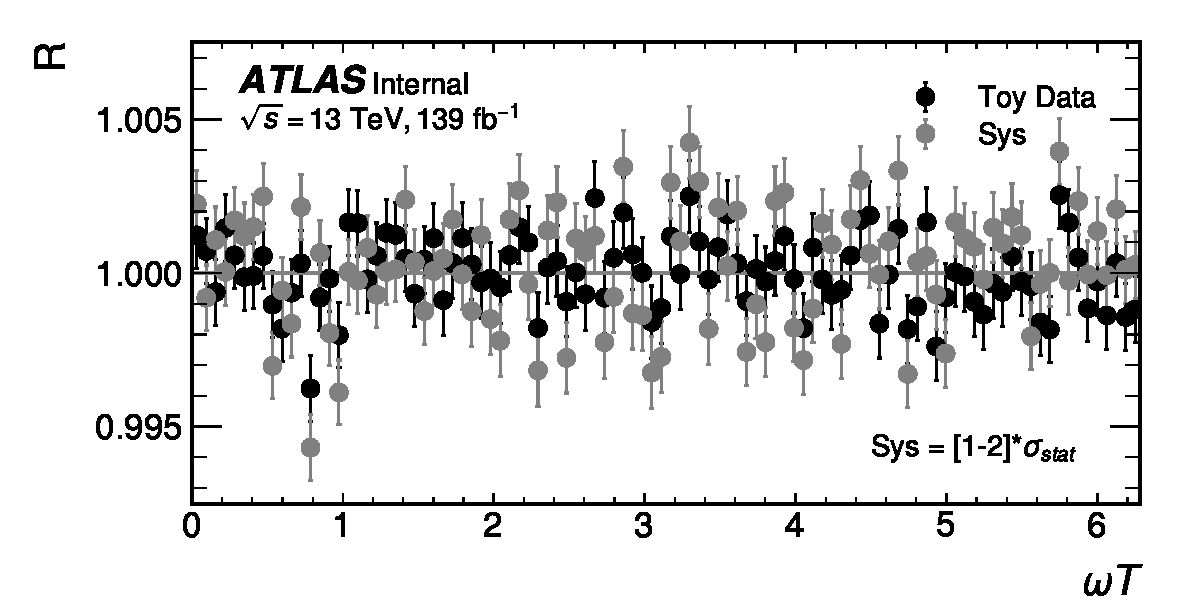
\includegraphics[width=0.45\textwidth]{figs/App_profile_chi2/profile_chi2_rnd_sys_PlusOneSigma_shifts}
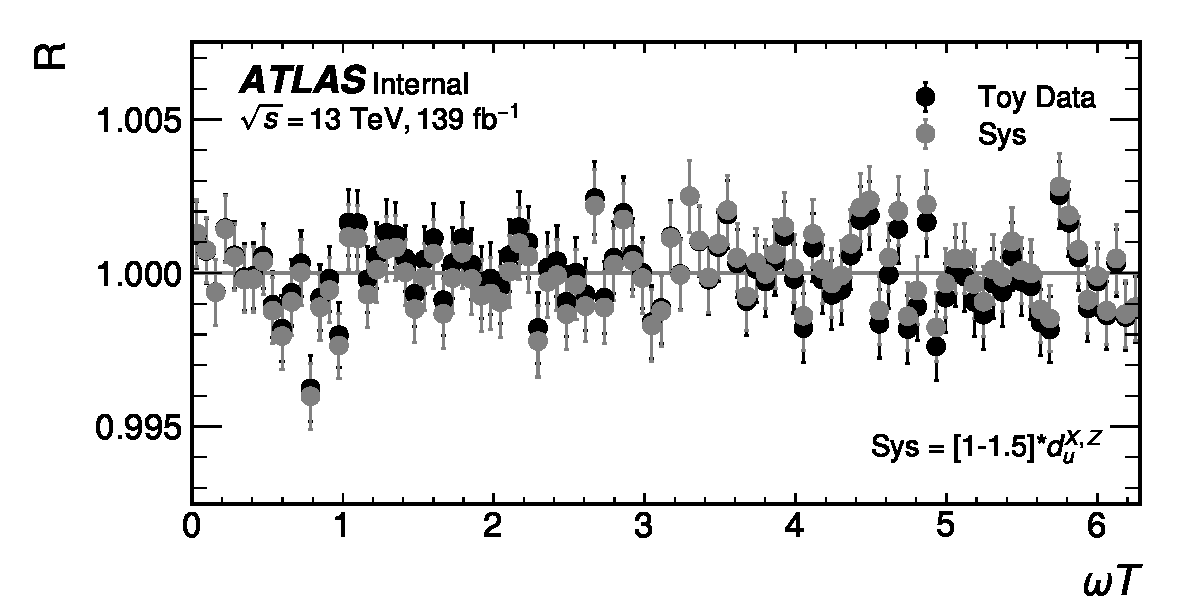
\includegraphics[width=0.45\textwidth]{figs/App_profile_chi2/profile_chi2_shape_sys_du_XZ_shifts}
\caption{The black color shows nominal data points, and the gray color shows shifted data points due to a systematic variation. The randomized systematic impacts top left (case 2). The systematic effect introduces a shape to data, top right (case 3)}
\label{fig:data_with_sys_shift}
\end{figure}



To test the profiled $\chi^{2}$ estimator, three cases for a set of systematic uncertainty are considered:

\begin{enumerate}
    \item $\beta = 0$. This is a default case where no systematic variations are included. This is for $\chi^{2}$ fit to the data points with black color in Figure~\ref{fig:data_with_sys_shift}, without profiling.
    
    \item $s_{i} = RandomChoise([-1,1])\times RandomNumber([1,2])\times \sigma_{i}$. Both the sign and size of $s_{i}$ are randomly chosen. Because we assume that the systematic impacts on data points are not correlated. 
    
    \item $s_{i} = RandomNumber([1,1.5])\times {d_{u}^{X,Z}}_{i}$. Add small signals to mimic shifts in data due to systematics. The size of $s_{i}$ is randomized between 1-1.5 times the signal in $ith$ point.
\end{enumerate}

Case 1 is one parameter $\chi^{2}$ fit since $\beta = 0$. To perform the profiled $\chi^{2}$ fit, $scipy$ python package is used (it is easier to implement in Python rather than in RooFit). The original $\chi^{2}$ fit in equation \ref{eq:chi2_estimator} is used to validate $scipy$ and $RooFit$ packages. Results from these two packages agreed very well up to high precision. 

In case 2, the size and sign of $s_{i}$ are randomly chosen so that they don't introduce some shapes (for example, cos- or sin-like oscillation). The $s_{i}$ are the difference between black and gray points in the left plot in Figure~\ref{fig:data_with_sys_shift}.

In case 3, the size and direction of shifts (sign) $\{s_{i}\}$ are introduced by a signal shape. The $d_{u}^{X,Z}$ is considered the shape, and the signal strength is set to $\mu = 1E^{-5}$. The $\{s_{i}\}$ are the difference between black and gray points in the right plot in Figure~\ref{fig:data_with_sys_shift}. As we can see in the plot, the shifts in data will introduce a signal-like shape to the dataset.


\begin{figure}
\centering
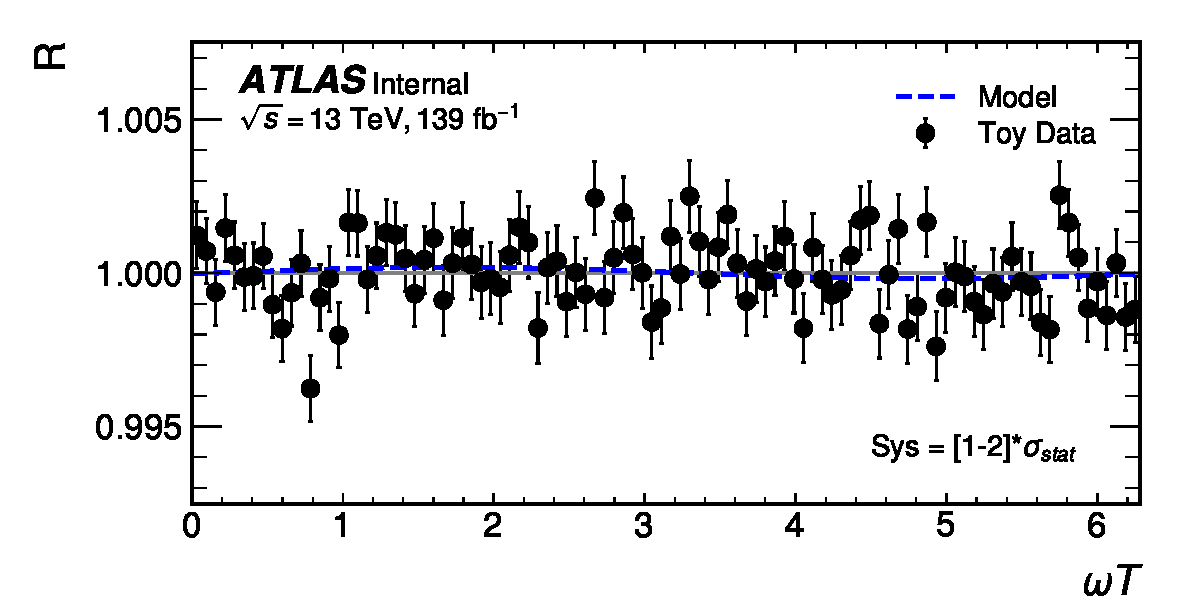
\includegraphics[width=0.45\textwidth]{figs/App_profile_chi2/profile_chi2_rnd_sys_PlusOneSigma_ToyData_postfit}
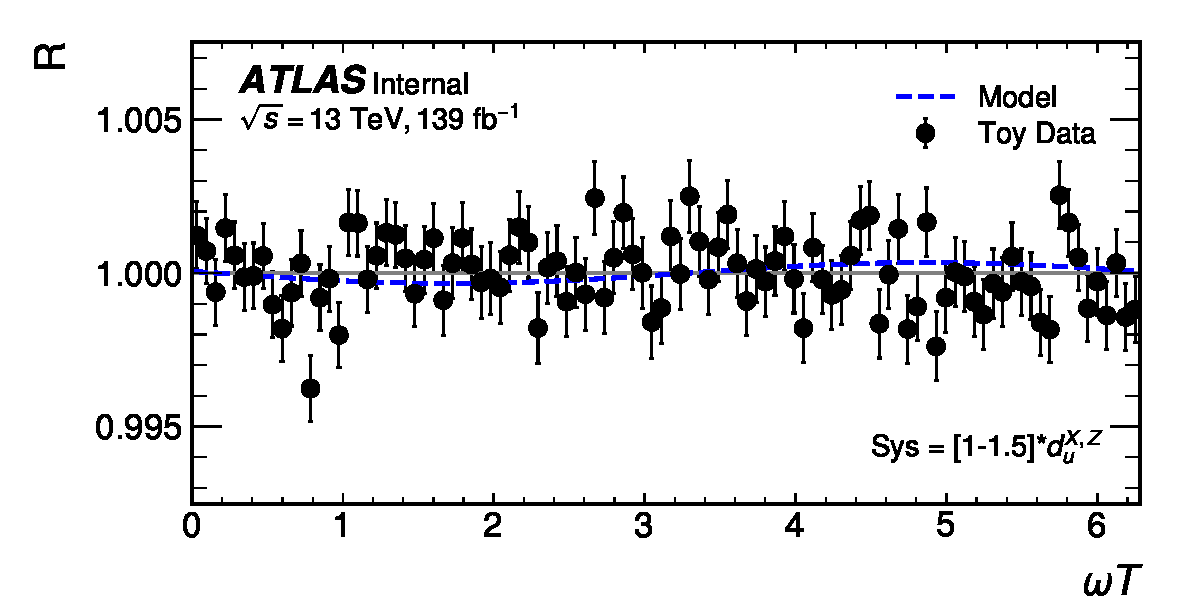
\includegraphics[width=0.45\textwidth]{figs/App_profile_chi2/profile_chi2_shape_sys_du_XZ_postfit}\\
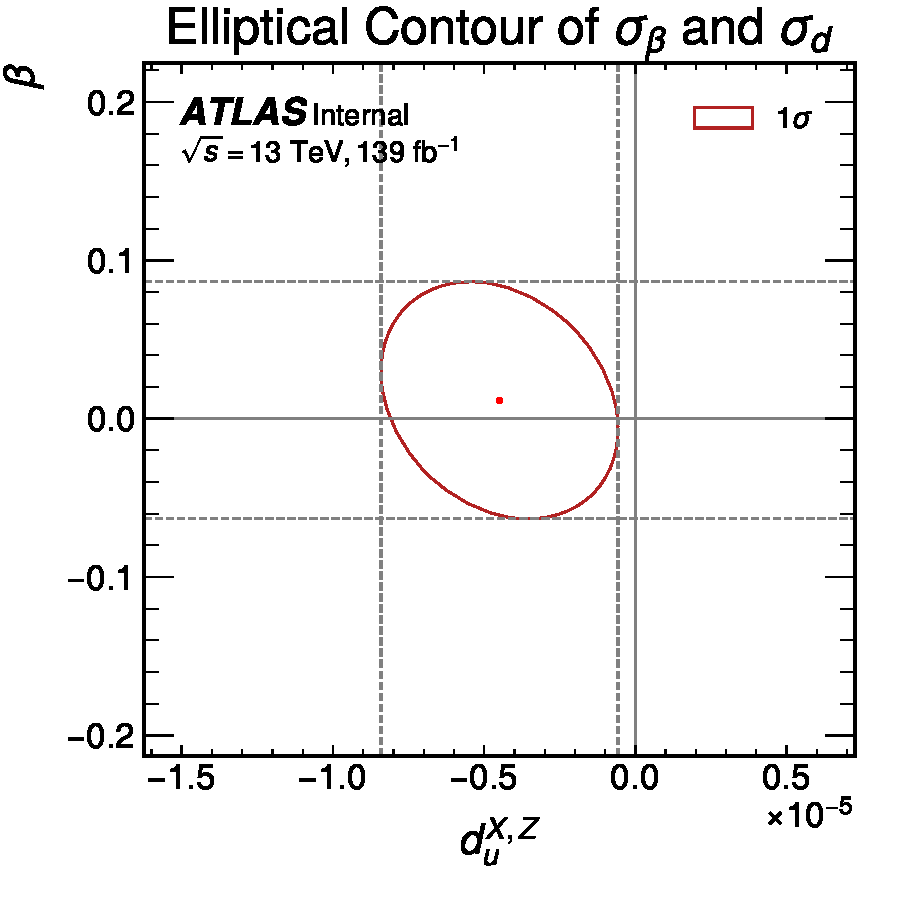
\includegraphics[width=0.45\textwidth]{figs/App_profile_chi2/profile_chi2_rnd_sys_du_XZ}
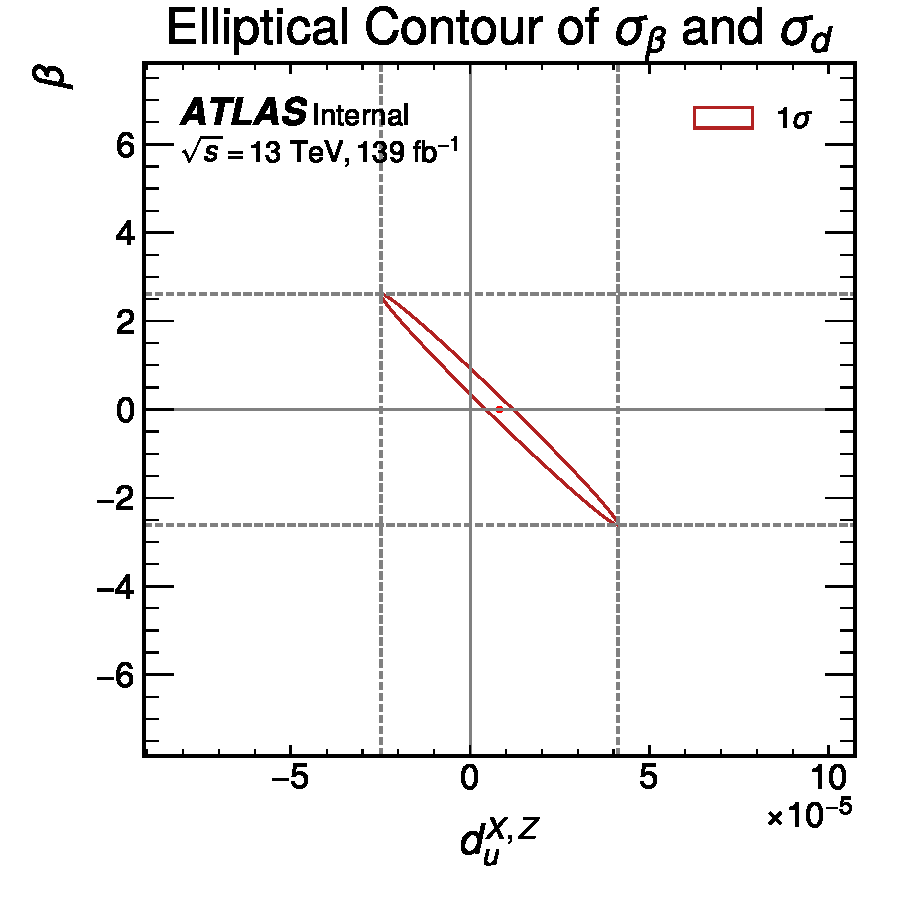
\includegraphics[width=0.45\textwidth]{figs/App_profile_chi2/profile_chi2_shape_sys_du_XZ}
\caption{Fit from the randomized systematic impacts top left (case 2). The fit with the systematics introduces a shape to data, top right (case 3). Corresponding one sigma contours from profiled $\chi^{2}(\beta, \mu)$ in the bottom plots.}
\label{fig:profile_chi2_fit_test}
\end{figure}

A profiled $\chi^{2}$ (Equition~\ref{eq:profile_chi2_estimator}) is fitted to Cases 2 and 3. The fit results are shown in Figure~\ref{fig:profile_chi2_fit_test}. The top left plot shows the toy data and fitted model (blue line). Since data is signal free and the systematic impact does not introduce any shapes to data, the fitted signal amplitude (or strength) is small. The bottom left plot shows the corresponding one-sigma contour. The input size for $\beta$ is [-1, 1] and it is constrained after the fit. The top right plot Figure~\ref{fig:profile_chi2_fit_test} shows the toy data and fitted model with profiled shape systematics (this systematic introduces signal like shape). From the corresponding contour plot (bottom right), one can see the impact of systematic uncertainty on the parameter estimation.

Fitted signal strength and its uncertainty from three cases are compared in Figure~\ref{fig:profile_chi2_fit_comparison}. The impact of the systematic is small for randomized uncertainty (Sys(rnd)) because this kind of systematics does not introduce oscillation shapes. The large impact is seen for a systematic that can introduce a signal-like shape (Sys(CORR)) to data.


\begin{figure}
\centering
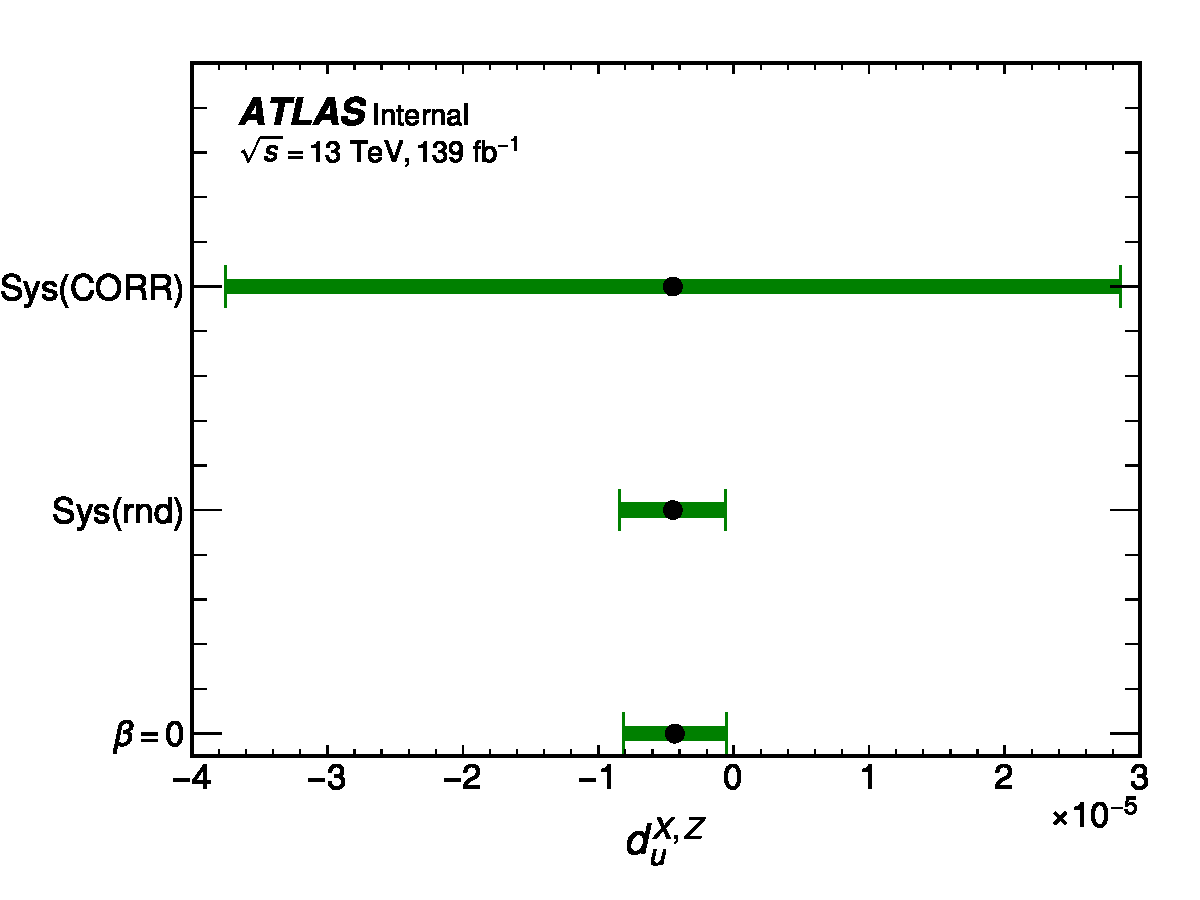
\includegraphics[width=0.6\textwidth]{figs/App_profile_chi2/profile_chi2_compare_fit_results}
\caption{Comparison of the fitted parameter $d_{u}^{X,Z}$ from $\chi^{2}$ ($\beta=0$) and profiled $\chi^{2}(\beta, \mu)$ fits using toy systematics in Case 2 (Sys(rnd)) and 3 (Sys(CORR)).}
\label{fig:profile_chi2_fit_comparison}
\end{figure}
 %% Ablet


